\documentclass{article}
\usepackage{graphicx, float}
\usepackage{listings}
\usepackage{xcolor}
\usepackage[left=1in, right=1in, top=0.25in, bottom=1in]{geometry}
\usepackage{caption, booktabs, subcaption}
\usepackage{sectsty, amsmath, amssymb, amsthm}
\usepackage{media9, hyperref, thmtools}





\usepackage{tikz}
\usetikzlibrary{intersections, calc, backgrounds}

\usepackage{pst-plot}
\usepackage{tikz-3dplot}
\usepackage{pgfplots}
\pgfplotsset{compat=1.18}


% small fix for canvas is xy plane at z % https://tex.stackexchange.com/a/48776/121799
\makeatletter
\tikzoption{canvas is xy plane at z}[]{%
    \def\tikz@plane@origin{\pgfpointxyz{0}{0}{#1}}%
    \def\tikz@plane@x{\pgfpointxyz{1}{0}{#1}}%
    \def\tikz@plane@y{\pgfpointxyz{0}{1}{#1}}%
    \tikz@canvas@is@plane}
\makeatother

\graphicspath{{./Images}}

\theoremstyle{definition}
\newtheorem{definition}{DEFINITION}


\title{MATH \& 254 QUADRIC SURFACES}
\author{Dharveen Suntheresen, Brendan Tea, Rohan Chilukuri}
\date{\today}



\begin{document}
\maketitle
\tableofcontents

\begin{abstract}
     Slicing a sliced hypercone results in 2D conic sections. Quadric Surfaces are slices of 4D hypercones resulting in 3D conics sections which are analogous to slices of 3D cones resulting in 2D conic sections. Hypercones allow one to derive quadrics surfaces. Knowing this lets students understand how quadric surfaces are related to each other and share the same innate properties. 
\end{abstract}

% https://drive.google.com/file/d/1UwYJcHtt1yPhnc7i-Lkt5ivxwfwJugNP/edit
\ \\ 
\ \\ 
\ \\ 
\ \\ 
\ \\ 


\begin{figure}[H]
        \centering
        \frame{\includegraphics[width=0.25\textwidth,height=0.25\textheight,keepaspectratio]{lukeyfeelingkindaquirky.png}}
        \caption[short]{Professor Luke Rawling - "Feeling kinda cute, might delete later"}
\end{figure}

\newpage
\section{Introduction}

\begin{definition}
Let $A,B,C,D,E,F,G,I,J \in \mathbb{R}$. Then, the 3D definition of a quadric surface is represented in the following form.
\begin{equation}
    A x^2 + B y^2 + C z^2 + D xy + E yz + F xz + G x + H y + I z + J = 0
\end{equation}
\end{definition}




Specific quadric surfaces are simplified forms of this general equation. For 2D conics sections , they are slices of 3D cones. By rotating a plane and changing its position, it will produce all of the conic sections: ellipses, parabolas, and hyperbolas. Using intuition reveals the geometric beauty of quadric surfaces: they are 3D slices of 4D objects.


\begin{figure}[h]
  \centering    

  \begin{subfigure}[b]{0.48\textwidth}
    \centering
    \includegraphics[width=\textwidth, keepaspectratio]{DoubleCone.png}
    \caption{Cone Quadric Surface}
    \label{fig:f1}
  \end{subfigure}
  \hfill
  \begin{subfigure}[b]{0.48\textwidth}
    \centering
    \tdplotsetmaincoords{70}{0}
\begin{tikzpicture}[declare function={radius(\x,\y,\z)=\z/(1+\y*cos(\x));
h(\x)=2.5*(2-\x);},scale=1.25,set scale/.code={\xdef\msc{#1}}]
 \begin{scope}[tdplot_main_coords]
  \begin{scope}[canvas is xy plane at z=0]
   \path[fill=orange!30] (0,0) circle (2);
   \coordinate (l) at (10:2);
   \coordinate (r) at (170:2);
   \draw[dashed,name path=back] (l) arc(10:170:2);
   \draw[thick,name path=front] (r) arc(170:370:2);
  \end{scope}
  \begin{scope}[on background layer]
   \draw[fill=orange!10] (l) -- (0,0,5) -- (r);   
  \end{scope}
  \path[name path global=coat] (l) -- (0,0,5) -- (r);   
  \pgfmathsetmacro{\meps}{0}
  %\pgfmathsetmacro{\msc}{0.75}
  \path[fill=blue] plot[variable=\x,domain=-180:180,samples=72,set scale=0.75] 
  ({radius(\x,\meps,\msc)*cos(\x)},
  {radius(\x,\meps,\msc))*sin(\x)},{h(radius(\x,\meps,\msc))});
  %\pgfmathsetmacro{\msc}{0.76}
  \fill[blue!60] plot[variable=\x,domain=170:370,samples=72,set scale=0.76] 
  ({radius(\x,\meps,\msc)*cos(\x)},
  {radius(\x,\meps,\msc))*sin(\x)},{h(radius(\x,\meps,\msc))})
  --
  plot[variable=\x,domain=370:170,samples=72,set scale=0.75] 
  ({radius(\x,\meps,\msc)*cos(\x)},
  {radius(\x,\meps,\msc))*sin(\x)},{h(radius(\x,\meps,\msc))})
  -- cycle  ;
  \pgfmathsetmacro{\meps}{0.15}
  \path[fill=green!30!black] plot[variable=\x,domain=-180:180,samples=72,set
  scale=1.25] 
  ({radius(\x,\meps,\msc)*cos(\x)},
  {radius(\x,\meps,\msc))*sin(\x)},{h(radius(\x,\meps,\msc))});
  \fill[green!70!black] plot[variable=\x,domain=170:370,samples=72,set
  scale=1.265]  ({radius(\x,\meps,\msc)*cos(\x)},
  {radius(\x,\meps,\msc))*sin(\x)},{h(radius(\x,\meps,\msc))})
  -- plot[variable=\x,domain=370:170,samples=72,set
  scale=1.25]  ({radius(\x,\meps,\msc)*cos(\x)},
  {radius(\x,\meps,\msc))*sin(\x)},{h(radius(\x,\meps,\msc))});
  \pgfmathsetmacro{\meps}{1.5}
  \path[fill=red!80!black] plot[variable=\x,domain=-70.6:70.6,samples=72,set
  scale=3] 
  ({radius(\x,\meps,\msc)*cos(\x)},
  {radius(\x,\meps,\msc))*sin(\x)},{h(radius(\x,\meps,\msc))});
  \path[fill=red!80] plot[variable=\x,domain=-70.6:10,samples=72,set
  scale=3]   ({radius(\x,\meps,\msc)*cos(\x)},
  {radius(\x,\meps,\msc))*sin(\x)},{h(radius(\x,\meps,\msc))})
  -- plot[variable=\x,domain=10:-69.6,samples=72,set
  scale=3.05]   ({radius(\x,\meps,\msc)*cos(\x)},
  {radius(\x,\meps,\msc))*sin(\x)},{h(radius(\x,\meps,\msc))})
  -- cycle;
  \pgfmathsetmacro{\meps}{4}
  \path[fill=orange!80!black] plot[variable=\x,domain=-51.4:51.4,samples=72,set
  scale=7] 
  ({radius(\x,\meps,\msc)*cos(\x)},
  {radius(\x,\meps,\msc))*sin(\x)},{h(radius(\x,\meps,\msc))});
  \path[fill=orange!60] plot[variable=\x,domain=-51.4:10,samples=72,set
  scale=7] 
  ({radius(\x,\meps,\msc)*cos(\x)},
  {radius(\x,\meps,\msc))*sin(\x)},{h(radius(\x,\meps,\msc))})
  -- plot[variable=\x,domain=10:-50,samples=72,set
  scale=7.15] 
  ({radius(\x,\meps,\msc)*cos(\x)},
  {radius(\x,\meps,\msc))*sin(\x)},{h(radius(\x,\meps,\msc))}) -- cycle;
 \end{scope}
\end{tikzpicture}
   
 \caption{3D Cone sliced into 2D Conic Sections}
  \end{subfigure}

  \caption{Cones and conics sections}
  \label{fig:both}
\end{figure}




\subsection{Horizontal Slices (3D Case)}
Let us start first with a rudimentary case that we are familiar with: a simple cone. Imagine a cone intersected by a simple horizontal plane. The plane $\mathbf{x = c}$, where $c \in \mathbb{R}$. Intersecting the cone $\mathbf{x^2 + y^2 = z^2}$ gives $\mathbf{c^2 + y^2 = z^2}$.



\begin{align}
&   (x-h)^2 + (y-k)^2 = (z-l)^2, \; \ \text{Set } x = C,  \\
&  1 = \frac{(z-l)^2}{c^2} + \frac{(y-k)^2}{c^2} 
\end{align}


\begin{figure}[H]
        \centering
        \frame{\includegraphics[width=0.25\textwidth,height=0.25\textheight,keepaspectratio]{hyperbolaslice.jpg}}
        \caption[short]{Slicing a 3d Cone results in a 2D Hyperbola}
\end{figure}

This is the equation of a hyperbola with an eccentricity of  $\frac{c}{a}=\frac{b\sqrt{{2}}}{b} = \sqrt{2}$ in this case. In general, substituting the plane equation into the cone eliminates the variable ($x$) and produces the boundary curve of the conic section.


%==================================================================
\subsection{Tilting \& Position Slices}

Generalizing this further, we can include an angle parameter alongside the position parameter to generate different conic sections. 





In the previous section, we examined horizontal slices of the cone 
\[
x^2 + y^2 = z^2,
\]
which produced hyperbolas. More generally, every conic section arises from 
intersecting this cone with a plane. The key geometric ingredient is the 
\emph{orientation} of the slicing plane, which is determined by its normal vector.

\begin{definition}
A plane in $\mathbb{R}^3$ can be written in normal form as
\[
n_x (x-d_x) + n_y (y-d_y) + n_z (z-d_z) = 0,
\]
where $\vec{\mathbf{n}} = \langle n_x, n_y, n_z \rangle$ is the normal vector of the plane and 
$d = (d_x,d_y,d_z)$ controls its position.
\end{definition}

The relationship between the plane's normal vector $\vec{\mathbf{n}}$ and the cone's axis 
determines which conic section appears.  
Without loss of generality, assume the cone
\[
x^2 + y^2 = z^2
\]
has axis parallel to the $z$-axis. Then the angle between the normal vector 
$\mathbf{n}$ and the cone axis $\mathbf{k} = (0,0,1)$ controls the shape of the 
intersection.

\begin{definition}
Let $\theta$ be the angle between the plane normal $\vec{\mathbf{n}}$ and the cone axis:
\[
\cos\theta = \frac{\mathbf{n}\cdot\mathbf{k}}{\|\mathbf{n}\|\|\mathbf{k}\|}.
\]
\end{definition}

The boundary between ellipses, parabolas, and hyperbolas is determined by comparing 
the plane's tilt angle to the cone's opening angle.  
For the cone $x^2 + y^2 = z^2$, the half-angle at the apex is $\alpha = 45^\circ.$\footnote{This is obtained from calculating the angle between the radius of the cone versus the height of z. Since $x^2 + y^2 = z^2$ will always have a 1:1 proportionality, $\arctan(\frac{r}{z}) = \arctan(\frac{1}{1}) = \frac{\pi}{4}$}

\begin{definition}
Let $\theta$ be the angle between the plane's normal vector and the cone axis.  
Then the intersection of the plane with the cone $x^2 + y^2 = z^2$ produces:
\begin{itemize}
    \item \textbf{Ellipse} \quad if $\theta < \alpha$ (the plane is ``steeper'' than the cone).
    \item \textbf{Parabola} \quad if $\theta = \alpha$ (the plane is parallel to a generator line of the cone).
    \item \textbf{Hyperbola} \quad if $\theta > \alpha$ (the plane is ``flatter'' than the cone).
\end{itemize}
\end{definition}

Geometrically, this means:
\begin{itemize}
    \item A plane whose normal is almost vertical cuts \emph{across} both sides of the cone 
          $\Rightarrow$ producing a hyperbola.
    \item A plane whose normal is tilted just enough to match the cone's slope touches 
          the cone along a single generator $\Rightarrow$ producing a parabola.
    \item A plane whose normal is sufficiently horizontal intersects only one nappe of the cone 
          $\Rightarrow$ producing an ellipse.
\end{itemize}

\subsubsection{Deriving the Conic Equation}




Given a plane with normal  $\vec{\mathbf{n}} = \langle n_x, n_y, n_z \rangle, \quad n_x x + n_y y + n_z z = d$.

\begin{align}
x^{2}+y^{2}
&= z^2\\
&= \left( \frac{d - n_x x - n_y y}{n_z} \right)^{2} \\[6pt]
&= \frac{d^{2} - 2dn_x x - 2dn_y y 
+ n_x^{2}x^{2} + 2 n_x n_y xy + n_y^{2}y^{2}}{n_z^{2}} \\[6pt]
n_z^{2}(x^{2}+y^{2}) 
&= d^{2} - 2dn_x x - 2dn_y y 
+ n_x^{2}x^{2} + 2 n_x n_y xy + n_y^{2}y^{2} \\[6pt]
0 &= 
(n_x^{2}-n_z^{2})x^{2}
+ (n_y^{2}-n_z^{2})y^{2}
+ 2 n_x n_y xy
- 2dn_x x
- 2dn_y y
+ d^{2} \\\
&= A x^2 + B xy + C y^2 + D x + E y + F
\end{align}

After expansion, the resulting equation is the standard form of a 2D conic section.  The coefficients and the discriminant $\Delta = B^2 - 4AC$ encode whether the curve is an ellipse ($\Delta < 0$), parabola ($\Delta = 0$), or hyperbola ($\Delta > 0$). Thus, by choosing the plane's normal vector, we may generate any desired conic section.



%-------------------------------------------------------------

\subsection{Extending this Idea Into 4D}

This pattern suggests a question: If 2D conic sections arise from "slicing" a 3D cone, what will happen when we "slice" the 4D analog of a cone? To answer this question, we shall apply the same method as used with 3D cones, but simply one dimension higher. Consider the equation for a 4D cone, sometimes referred to as a hyper cone.

\begin{definition}
Let $A,B,C \in \mathbb{R}$ \text {and}  $(h,k,m,n)$ be a point on the graph . Then, let a hyper cone be represented by the following.

\begin{equation}
    A(x-h)^2 + B(y-k)^2 + C(z-l)^2 = (w-m)^2
\end{equation}

\end{definition}



Okay, with this, let us extend this idea see what happens when we apply this same idea. This is the direct 4D analog of the familiar 3D cone.
Given we can make all the quadric surface with a standard hyper cone, we will be referring to the equation $\mathbf{x^2 + y^2 + z^2 = w^2}$ as our sample hyper cone for the rest of the paper. If we “slice" the sample hyper cone with the 3D hyperplane at $\mathbf{w=c}$ where $c \in \mathbb{R}$ and substitute it into the hyper cone equation, we get back to the equation of a circle.



\begin{equation}
    x^2 + y^2 + z^2 = c^2
\end{equation}


Intersecting a $n$-dimensional object with an $(n-1)$-dimensional slice produces a $(n-1)$-dimensional cross-section. This applies quadric surfaces too, slicing any quadric surface can give us the 2D conic section equivalent.
\ \\
\ \\
\ \\ 
\

\begin{figure}[h]
    \centering
   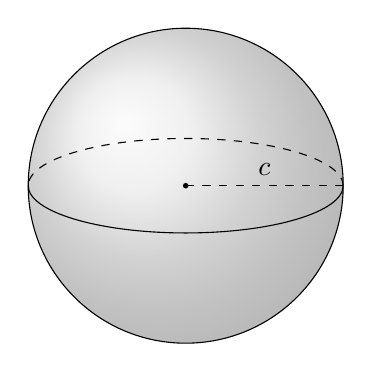
\begin{tikzpicture}
  \shade[ball color = gray!40, opacity = 0.4] (0,0) circle (2cm);
  \draw (0,0) circle (2cm);
  \draw (-2,0) arc (180:360:2 and 0.6);
  \draw[dashed] (2,0) arc (0:180:2 and 0.6);
  \fill[fill=black] (0,0) circle (1pt);
  \draw[dashed] (0,0 ) -- node[above]{$c$} (2,0);
\end{tikzpicture}
    \caption{Circle with radius $c$}
    \label{fig:placeholder}
\end{figure}

\section{Types of Quadric Surfaces}

In the same way we take hyperplanes, we can also take titled hyperplanes with specific angles. Each specific angle has a different intersection that produces different quadric surfaces. For a standard hypercone with no coefficients on its dimensions, the following angles will produce:


\begin{itemize}
    \item $\theta \geq 45^\circ$: Unbounded Cross Section $\Longrightarrow$ Hyperboloid
    \item $0^\circ \leq \theta < 45^\circ$: Bounded Cross Section $\Longrightarrow$ Ellipsoid
    \item $\theta = 45^\circ$: Conic Degeneration $\Longrightarrow$ Paraboloid
    \item $\theta = 0^\circ$: Perpendicular Bounded Cross Section $\Longrightarrow$ Sphere
\end{itemize}


% \begin{align}
%     & z^2 = y^2 \\
%     & |z| = |y| \\
% \end{align}


We can classify these quadric surfaces into two categories: generate and degenerate quadrics. Through connecting linear algebra with calculus, we can obtain the quadric surfaces into a matrix form. 

\begin{definition}
A quadric surface can be defined with the following. 

\begin{align}
& \text{Let} X = \begin{bmatrix} x \\ y \\ z \\ 1 \end{bmatrix} ,\quad 
    Q = \begin{bmatrix}
    J & G/2 & E & I/2 \\
    G/2 & A & D/2 & E/2 \\
    H/2 & D/2 & B & F/2 \\
    I/2 & E/2 & F/2 & C
\end{bmatrix}, \quad Q_3 =
\begin{bmatrix}
 J & G/2 & E \\
G/2 & A & D/2 \\
H/2 & D/2 & B
\end{bmatrix}. \\ 
& \boxed{X^T Q X = 0}
\end{align}

\end{definition}

\begin{definition}

\begin{align}
& \text{A degenerate quadric surface is when} \det(Q_3) \ne 0. \\
& \text{A generate quadric surface is when} \det(Q_3) = 0.
\end{align}

\end{definition}


\begin{figure}[h]
    \centering
    \includegraphics[width=0.8\linewidth]{Possible-quadric-surfaces-built-from-the-intersection-of-a-hypercone-with-a-hyperplane.png}
    \caption{Possible quadric surfaces}
    \label{fig:placeholder}
\end{figure}

%-----------------------------------------
\newpage
\subsection{Spheres \& Ellipsoid}

\begin{figure}[h]
    \begin{minipage}{0.49\textwidth}
     As previously discussed, one can get a sphere by setting the hyperplane cross section to $w=c$. If one rotates the hyperplane intersecting the hyper cone less than when it may exceed an angle of $\frac{\pi}{4}$ they can distort the section giving an ellipsoid.

Ellipsoid equation:
Set $w = (Ax+ By+ Cz + c)$ where it to generates a hyperplane whose angle from the central cross section of the hyper cone is less than $\frac{\pi}{4}$. 

\begin{equation}
    A(x-h)^2 + B(y-k)^2 + C(z-l)^2 = w
\end{equation}

    \end{minipage}
    \hfill
    \begin{minipage}{0.5\textwidth}
        \centering
        \includegraphics[width=\textwidth,keepaspectratio]{2560px-Ellipsoide.png}
        \caption{A sphere and different distortions of it creating ellipsoid variants}
    \end{minipage}
\end{figure}
%--------------------------------------------------
\subsection{Elliptic \& Hyperbolic Paraboloid}

One can make an elliptic paraboloid in the same way except have the angle between the central cross section and the hyperplane w is set to to be $\frac{\pi}{4}$.
\begin{figure}[h]
    \centering
    \includegraphics[width=0.2\linewidth]{Paraboloid_of_Revolution.svg.png}
    \caption{Elliptic Paraboloid in a 3D Space}
    \label{fig:stuff}
\end{figure}
% \subsection{Hyperboloid of One \& Two Sheets}
% A hyperboloid of 2 two sheets can be obtained by choosing a linear tilted hyperplane

% Start with the equation for a 4D hyper cone
% \begin{equation}
%     x^2 + y^2 + z^2 = w^2
% \end{equation}

% Intersect this hyper cone with a hyperplane by making the substitution

% \begin{equation}
%     w=(ac+d)
% \end{equation}

% By now we have established that taking a cross sections of a hyper cone generates quadric surfaces. 
% (maybe include)

% \begin{figure}[h]
%     \centering
%     \includegraphics[width=0.3\linewidth]{250px-Hyperboloid2.png}
%     \caption{Hyperboloid of Two Sheets in a 3D space}
%     \label{fig:placeholder}
% \end{figure}


% \subsection{Weird hyperplane cross section Cases}

% \subsubsection{Elliptic Cone}
% \subsubsection{Elliptic Cylinder}
% \subsection{Cone}

% \subsection{Hyperboloid of One Sheet}

% \begin{figure}[h]
%     \centering
%     \includegraphics[width=0.3\linewidth]{Hyperboloid1.png}
%     \caption{Hyperboloid of One Sheet in a 3D space}
%     \label{fig:placeholder}
% \end{figure}



% \includemedia[
%   activate=onclick,
%   width=300pt, height=200pt,
%   3Dtoolbar, label=3d_model.u3d % Path to your U3D file
% ]{}{3d_model.u3d}

\section{Conclusion}

By noticing patterns in math through a geometric lens and applying them across dimensions, we reveal underlying properties that unify ideas which seem unrelated. We recapped how conic sections are created from intersecting a plane with a 3D cone at varying angles, which produces circles, ellipses, parabolas, and hyperbolas. Once we extended this idea into the 4th dimension we can see that all quadric surfaces are related to the cross sections of a 4D hyper cone. The type of quadric surface obtained is dependent on the orientation and position of of the intersecting hyperplane. This is the direct 3D equivalent of eccentricity found in conic sections.

% \section{Conclusion}

By noticing patterns in math through a geometric lens and applying them across dimensions, we reveal underlying properties that unify ideas which seem unrelated. We recapped how conic sections are created from intersecting a plane with a 3D cone at varying angles, which produces circles, ellipses, parabolas, and hyperbolas. Once we extended this idea into the 4th dimension we can see that all quadric surfaces are related to the cross sections of a 4D hyper cone. The type of quadric surface obtained is dependent on the orientation and position of of the intersecting hyperplane. This is the direct 3D equivalent of eccentricity found in conic sections.

\end{document}
